\pagestyle{plain}

\chapter{Problemas da Mochila} \label{sec:mochila}

Existem diversas versões de Problemas da Mochila, todos elas caracterizadas por selecionar, dentre um conjunto de objetos ou itens disponíveis, um subconjunto que irá otimizar uma função objetivo, satisfazendo determinadas restrições. Para tanto, cada item deve possuir um {\it ``peso''} e um {\it ``benefício''}. Por peso entende-se uma penalidade a ser paga pela inclusão do item. É comum encontrar o termo ``penalidade'' ou ``custo'' para expressar o peso de um item. Por ``benefício'' entende-se a utilidade ou lucro obtido pela escolha do item e esse valor contribuirá no objetivo do problema. 

A principal restrição imposta nos problemas da mochila relaciona-se à sua capacidade. De fato, a soma do peso dos itens selecionados deve respeitar a capacidade da mochila. Geralmente, expressamos capacidade da mochila e custo dos itens utilizando a mesma unidade de medida. Várias outras restrições ou condições podem ser impostas no problema e cada nova restrição agrega um custo computacional para encontrar sua solução. O Problema da Mochila, em sua versão mais simples, é integrante da classe NP-difícil \cite{GJ79}. Consequentemente, várias outras versões do Problema da mochila, várias delas apresentadas nesse texto, pertencem também à mesma classe de problemas.

Neste capítulo são apresentadas várias classes de Problemas da Mochila, incluindo descrição e modelo matemático, com o objetivo de ilustrar a diversidade de problemas relacionados. Essa fundamentação será útil para que nos próximos capítulos seja estudada a versão de Problemas da Mochila de maior interesse neste trabalho, conhecida como Problema da Mochila Compartimentada. Ainda no capítulo veremos os principais métodos e técnicas de resulução computacional dos problemas da mochila, incluindo alguns algoritmos para exemplificação. 

\section{Classes de Problemas da Mochila}

Todas as mochilas que serão apresentados nessa seção utilizam um conjunto de itens $S$ com $n$ itens, cada item $i$ ($1 \leq i \leq n$) deve estar associado a um valor de benefício $b_i$ e um peso $l_i$. A capacidade da mochila é representada por $L$. 


\subsection{Problema da Mochila 0-1} \label{m01}

Para cada item $i \in S$ é associada a variável $x_i$ que pode assumir um dos dois valores: 0 ou 1. $x_i$ será 0 quando o item $i$ não for escolhido para compor a mochila, e será 1 quando o item fizer parte da solução. Por esse motivo, essa versão também é conhecida como mochila binária. Segue abaixo o modelo matemático:

\hspace*{3.0cm} Maximize:
\begin{equation}
 \sum_{i=1}^n b_i x_i 
\end{equation} 

\hspace*{3.0cm} Sujeito a:
\begin{equation}
 \sum_{i=1}^n l_i x_i  \leq L
\end{equation} 

\begin{equation}
 x_i=0 \textrm{ ou } 1, i=1,...,n 
\end{equation} 

Algumas informações com relação ao conjunto de itens podem ser observadas. Por exemplo, nenhum item do conjunto $S$ deve possuir peso maior do que a capacidade máxima da mochila, pois, caso contrário, esse item não faria parte de nenhuma solução do problema. Outro ponto importante sobre o conjunto de itens é que a soma dos pesos dos itens de $S$ não pode ser menor que $L$, já que desta forma a solução ótima seria a soma dos benefícios de todos os itens. 

\subsection{Versão Fracionária do Problema da Mochila} \label{frac}

Se não houver a restrição de {\it aceitar} ou {\it recusar} um item de $S$ para fazer parte da solução, e tivermos a possibilidade  de escolher uma porção do item para fazer parte da solução, teremos a versão fracionária do Problema da Mochila. Nessa versão, permite-se escolher pedaços arbitrários de alguns elementos. Deseja-se, então, encontrar a porção $x_i$ do item $i$ que fará parte da solução, tal que

\begin{equation}
 0 \leq x_i \leq l_i \textrm{ para cada } i\in S \textrm{ e } \sum_{i=1}^n x_i \leq L 
\end{equation}

O benefício total do conjunto de itens é determinado pela função objetivo

\begin{equation}
 \sum_{i \in S} b_i(x_i/l_i)
\end{equation}

Essa versão do problema possui uma solução bastante simples utilizando a abordagem gulosa, ordenando o conjunto de itens pelo valor $b_i/l_i$ e fazendo com que os itens com maior valor $b_i/l_i$ sejam escolhidos primeiro até que não seja mais possível incluir um item por completo. Seja $j$ $(0 \leq j \leq n)$ o último item avaliado e inserido por completo na solução e seja $l$ o somatório dos pesos dos itens já inseridos até o momento.  A porção do item $j+1$, se tal item existir, que fará parte da solução será $x_{j+1} = L-l$. 

Por ter uma solução polinomial bastante simples, esta versão do problema não se enquadra na classe de problemas que estamos estudando neste trabalho. Porém, na seção ~\ref{bb}, utiliza-se a abordagem gulosa descrita acima em um método heurístico para cálculo de um limitante superior para o valor da solução ótima, que será utilizado em um algoritmo {\it branch and bound} para solucionar do Problema da Mochila 0-1. 



\subsection{Problema da Mochila Restrita}

Na classe de mochilas restritas, as variáveis deixam de ser binárias e passam a indicar o número de repetições do respectivo item na mochila. Além do mais, cada variável têm associada a ela um limitante inferior e um superior. No modelo matemático desta classe, $d_i$ e $t_i$ representam o limitante superior e o limitante inferior para o item $i$, respectivamente. 

\hspace*{3.0cm} Maximize:
\begin{equation}
 \sum_{i=1}^n b_i x_i 
\end{equation} 

\hspace*{3.0cm} Sujeito a:
\begin{equation}
 \sum_{i=1}^n l_i x_i  \leq L
\end{equation} 

\begin{equation}
 t_i \leq x_i \leq d_i \textrm{ e inteiro }, i=1,...,n 
\end{equation} 

Por questões de simplicidade, pode ser necessário definir o limitante inferior como zero. Dado um problema definido como no modelo anterior, basta somar $(t_i*t_i)$ na função objetivo, subtrair $(l_i * t_i)$ de $L$ e $t_i$ de $d_i$, e finalmente, atualizarmos $t_i$ para zero. Com essa simples transformação sempre teremos zero como limitante inferior. 

Outra observação importante é que toda mochila restrita pode ser transformada em uma mochila 0-1. Um método para realizar essa transformação é ilustrado por~\cite{MT90}.

\subsection{Problema da Soma de Subconjuntos}

Esse tipo de mochila se aproxima muito da classe de mochilas com variáveis binárias. A diferença se restringe à função objetivo onde o benefício é substituído pelo peso do item. Esta nova abortagem é útil quando é necessário selecionar um subconjunto de itens, cuja soma de seus pesos se aproxime ao máximo, mas não exceda, a capacidade da mochila.  Segue o modelo matemático equivalente:

\hspace*{3.0cm} Maximize:
\begin{equation}
 \sum_{i=1}^n l_i x_i 
\end{equation} 

\hspace*{3.0cm} Sujeito a:
\begin{equation}
 \sum_{i=1}^n l_i x_i  \leq L
\end{equation} 

\begin{equation}
 x_i=0 \textrm{ ou } 1, i=1,...,n 
\end{equation} 

Esse problema pode surgir, por exemplo, nessas circunstâncias: considere um servidor de internet e um conjunto de pedidos de download. Para cada pedido de download, podemos determinar o tamanho do arquivo solicitado e, por isso, podemos sintetizar cada pedido como um valor inteiro (representando o tamanho do arquivo solicitado). Dado esse conjunto de inteiros, pode ser interessante determinar um subconjunto deles que, quando somados, tenham a largura de banda de nosso servidor durante uma fração de tempo. Esse problema é uma instância do problema da soma de subconjuntos. 

Infelizmente, fica mais difícil resolver esse problema à medida que a largura de banda e a capacidade de atender pedidos aumentam. Esse é um problema da classe NP-completo e a demonstração de que, de fato, pertence a esta classe de problemas encontra-se em~\cite{MTG02}.

\subsection{Problema de Múltiplas Mochilas 0-1}

No Problema de Múltiplas Mochilas considera-se $n$ conjuntos de itens, disjuntos entre si, e um conjunto com $m$ mochilas, cada uma com capacidade $L_j$ $(1 \leq j \leq m)$. O problema consiste em atribuir itens que fornecerão o maior benefício possível, considerando que os itens de um determinado conjunto podem ser atribuídos a, no máximo, uma única mochila. Nesse caso, a variável de decisão $x_{ij}=1$, se o item $i$ foi adicionado à mochila $j$. Caso contrário, $x_{ij}=0$. 

\hspace*{3.0cm} Maximize:
\begin{equation}
 \sum_{j=1}^m \sum_{i=1}^n b_i x_{ij} 
\end{equation} 

\hspace*{3.0cm} Sujeito a:
\begin{equation}
 \sum_{i=1}^n l_i x_{ij} \leq L_j, j=1,...,m
\end{equation} 

\begin{equation}
 \sum_{j=1}^m x_{ij} \leq 1, i=1,...,n
\end{equation} 

\begin{equation}
 x_{ij}=0 \textrm{ ou } 1, i=1,...,n , j=1,...,m 
\end{equation} 

Quando $n=1$, o Problema de Múltiplas Mochilas 0-1 se reduz a um Problema da Mochila 0-1 original.


\section{Estratégias para Resolução de Mochilas} \label{cap2_tec_estr}

Embora o Problema da Mochila 0-1 e suas variações sejam pertencentes à classe NP-difícil, muitos deles surgem em aplicações práticas na vida real ou como sub-problemas de outros problemas mais complexos e por isso justifica-se a tentativa de encontrar soluções exatas ou aproximadas, mesmo que isso custe muito tempo. Nesta seção abordaremos as principais técnicas de projeto de algoritmos utilizadas para resolver de maneira exata ou aproximada alguns Problemas da Mochila. 

\subsection{Branch and Bound} \label{bb}

Esta técnica apresenta-se como um método geral para encontrar soluções ótimas para problemas de otimização combinatória. Esse método tem como entrada uma instância para um problema difícil de otimização e como saída uma solução ótima, se existir. A estratégia usando força-bruta é buscar sistematicamente em um grande (possivelmente exponencial) conjunto de possibilidades, computar o valor associado a cada possível configuração e devolver a melhor das configurações encontradas de acordo com uma função objetivo de maximização ou minimização. A técnica {\it branch-and-bound} utiliza o mesmo método, porém inclui um mecanismo para diminuir o conjunto de possibilidades, descartando a verificação daquelas configurações que não tenham chance de serem soluções ótimas, melhorando o tempo de resposta do algoritmo. Para descartar configurações não promissoras, calcula-se um {\it limitante} que é o valor máximo (para problemas de maximização) ou mínimo (para problemas de minimização) que uma solução pode atingir a partir da configuração em questão. Se esse valor limitante não for satisfatório, essa configuração  (e consequentemente, todas que seriam atingidas no espaço de busca a partir dela) será descartada. A dificuldade inerente a esta técnica está no fato de que quanto melhor for definido o limitante, melhor o tempo de resposta do algoritmo.

Para explicar como aplicar a técnica {\it branch and bound},  considera-se, nesse contexo, o Problema da Mochla 0-1, descrita na subseção ~\ref{m01}. Um limitante será definido utilizando uma abordagem gulosa, similar à técnica utilizada para resolver a versão fracionária do Problema da Mochila, descrita na seção ~\ref{frac}. Assume-se que os itens do conjunto $S$ sejam colocados em ordem não-decrescente, pelo valor de $b_i/l_i$. Eles serão processados nesta ordem, pois assim estaremos considerando os itens na ordem de benefício/custo decrescente, começando com o elemento de maior benefício/custo. Nossa configuração é definida pelo subconjunto $S_i$ dos primeiros $i$ itens de $S$ baseados nesta ordem. Assim, os índices dos itens de $S_i$ estão entre 0 e $i-1$, e podemos definir o conjunto $S_0$ como uma configuração vazia. 

Iniciamos colocando a configuração $S_0$ em uma fila de prioridades $P$ e, a cada iteração do algoritmo, escolhemos a configuração mais promissora $c$ em $P$. Se $i$ é o índice do último item considerado em $c$, então expandimos $c$ em duas novas configurações: uma que inclui o item $i+1$ e uma que não o inclui. Note que cada configuração satisfatória à restrição de tamanho é uma configuração válida para o problema em questão. Assim, se qualquer uma das duas configurações for válida e melhor do que a melhor solução encontrada até o momento, atualizamos nossa melhor opção corrente e continuamos o processo. 

Para escolher configurações que sejam mais promissoras, precisamos ter uma forma de avaliá-las por seu valor potencial. Para tanto, utilizaremos um limite superior para o seu valor potencial: dada uma configuração $c$ que considera os itens de índice $0$ a $i$, calculamos um limite superior para $c$ iniciando com o valor total $l_c$ de $c$ e verificando quanto valor a mais podemos colocar em $c$ se aumentarmos $c$ com uma solução para o problema fracionário da mochila que seja retirada dos itens restantes em $S$. Seja $k$ o maior índice tal que $\sum_{j=i+1}^{k} s_j \leq L-s_c$, onde $s_c$ é o somatório dos pesos de todos os itens que compõem na configuração $c$. Os itens de $i+1$ a $k$ são os melhores itens que ainda cabem na mochila. Para calcular o limite superior para $c$, consideramos a adição de todos esses elementos a $c$ mais tudo o que for possível do item $k+1$ (se existir). Nosso limite superior $upper(c)$ para $c$ será então definido como segue:


\begin{equation}
 upper(c)= l_c+ \sum_{j=i+1}^{k} l_j + (L-s_c-\sum_{j=i+1}^{k} s_j) (l_{k+1})/(s_{k+1})
\end{equation} 

Se $k=n-1$, então assumimor que $(l_{k+1})/(s_{k+1}) = 0$.

No capítulo seguinte mostraremos os resultados obtidos por meio da implementação da técnica descrita para solucionar o Problema da Mochila 0-1 utilizando {\it branch-and-bound} e avaliaremos seu desempenho com relação aos outros métodos implementados.



\subsection{Programação Dinâmica} \label{progdin}


A proposta mais simples e promissora para resolver o Problema da Mochila 0-1 é utilizar programação dinâmica. Inicialmente, os itens de $S$ serão numerados como 1,2,3,...,$n$ e para cada $k \in \{1,2,...,n\}$, defini-se $S_k$ como o subconjunto contendo itens $S$ rotulados de 1 até $k$.

Formulamos, então, cada subproblema como sendo o cálculo de $B[k,w]$, que é definido como o valor total máximo (benefício total) de um subconjunto
$S_k$ entre todos os subconjuntos que têm seus pesos totais até $w$. Teremos $B[0,w]$=0 para cada $w \leq W$ e derivaremos a seguinte
relação para o caso geral:


\[ B[k,w]= \left \{ \begin{tabular}  {lc}
                                     $B[k-1,w]$ & $:l_k > w$ \\
                                     $max\{ B[k-1,w], B[k-1,w-l_k]+b_k\}$ & $:l_k \leq w$ \\
                                  \end{tabular} \right. \]


Ou seja, $B[k,w]$ é o melhor subconjunto $S_k$ cujo peso total $w$ é ou o melhor subconjunto de $S_{k-1}$ que tem o peso total $w$ ou o melhor
subconjunto de $S_{k-1}$ que tem peso total $w-l_k$ mais o item $k$. Uma vez que o melhor subconjunto de $S_k$ com o peso total $w$ deva ou não conter o item $k$, uma dessas duas escolhas será a melhor.

\begin{algorithm}
\caption{Mochila\_Programção\_Dinâmica} %titulo do algoritmo
\label{alg2}
\begin{algorithmic}[1]
 
	\REQUIRE Conjunto $S$ de $n$ itens, tais que o item $i$ tem um benefício positivo $b_i$ e um peso inteiro positivo $l_i$, um inteiro positivo $L$ que corresponde ao peso total da mochila.
 
	\ENSURE Para $w=0,...,L$, o benefício máximo $B[w]$ de um subconjunto de $S$ com peso total $w$.

	\FOR {$w \leftarrow 0$ \ até \ $L$}
		\STATE $B[w] \leftarrow 0$
	\ENDFOR
	\FOR {$k \leftarrow 1$ \ até \ $n$}
		\FOR{$w \leftarrow L$ \ descrescendo \ até \ $l_k$}
			\IF{$B[w-l_k]+b_k > B[w]$}
				\STATE $B[w] \leftarrow B[w-l_k]+b_k$
			\ENDIF
		\ENDFOR
	\ENDFOR
\end{algorithmic}
\end{algorithm}

O tempo de execução do algoritmo é determinado pelos dois laços aninhados, onde o mais externo tem $n$ iterações e o mais interno tem no máximo $L$ iterações. Desta forma, poderemos determinar o valor ótimo localizando o maior entre todos os elementos do vetor $B$. Assim, podemos encontrar o subconjunto de $S$ de maior benefício com peso total de no máximo $L$ em tempo $O(nL)$. 

Considera-se que é um algoritmo de complexidade de tempo pseudo-polinomial, já que depende, além da quantidade de itens do conjunto $S$, da magnitude de um número fornecido na entrada. Porém, na prática, esse algoritmo comporta-se muito melhor do que o algoritmo de força bruta (exponencial). No capítulo seguinte mostramos os resultados referentes à implementação desse método e avaliaremos o seu desempenho com relação aos outros métodos também implementados.


\subsection{Algoritmos Genéticos} \label{algen}

Os algoritmos genéticos são uma família de modelos computacionais inspirados na evolução, indicados para encontrar soluções aproximadas para problemas de otimização difíceis, como o Problema do Caixeiro Viajante, Problemas de Satisfabilidade ou Problemas da Mochila, que envolvem um grande número de variáveis e, consequentemente, espaços de soluções de dimensões elevadas ~\cite{Wei09}. Nesta seção, mostraremos os conceitos relacionados a esta técnica a fim de fundamentar a proposta de um algoritmo genético para encontrar uma solução aproximada para o Problema da Mochila 0-1 e sua extensão para o Problema da Mochila Compartimentada.

Embora existam variações de acordo com a aplicação, algoritmos genéticos simples normalmente trabalham com descrições de entrada formadas por cadeias de bits de tamanho fixo.  Há três tipos de representação possíveis: binária, inteira ou real. A essa representação se dá o nome de {\it alfabeto} do algoritmo. De acordo com a classe de problema que se deseje resolver pode-se usar qualquer um dos três tipos. Neste trabalho, utilizaremos alfabeto binário. 

Uma implementação de um algoritmo genético começa com uma população aleatória de cromossomos. Essas estruturas são, então, avaliadas e associadas a uma probabilidade de reprodução de tal forma que as maiores probabilidades são associadas aos cromossomos que representam uma melhor solução para o problema de otimização do que àqueles que representam uma solução pior.

Os principais conceitos envolvidos na implementação de algoritmos genéticos que foram utilizados para elaboração de um algoritmo genético para solucionar Problemas da Mochila neste trabalho são:
\begin{itemize}
\item {\bf gene:} um ou mais símbolos do alfabeto (neste trabalho, um gene corresponde a um símbolo do alfabeto binário)
\item {\bf cromossomo:} conjunto de genes que corresponde a um indivíduo
\item {\bf população:} conjunto de cromossomos (ou indivíduos) que corresponde ao conjunto de pontos no espaço de busca 
\item {\bf geração:} iteração completa do algoritmo genético que gera uma nova população 
\item {\bf aptidão bruta:} saída gerada pela função objetivo para um indivíduo da população 
\item {\bf aptidão máxima:} melhor aptidão encontrada para indivíduos da população corrente 
\item {\bf aptidão média:} aptidão média da população corrente 
\end{itemize}

Deve ser observado que cada cromossomo, chamado de indivíduo no algoritmo, corresponde a um ponto no espaço de soluções do problema de otimização. O processo de solução adotado nos algoritmos genéticos consiste em gerar, através de regras específicas, um grande número de indivíduos (população), de forma a promover uma varredura tão extensa quanto necessária do espaço de soluções. 

\begin{figure}[htp]
	\centering
	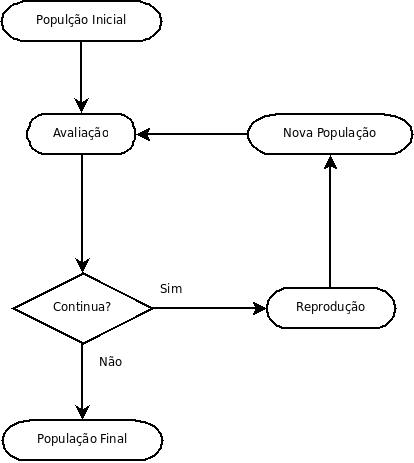
\includegraphics[scale=0.5]{images/fluxo.jpg}
	\caption{Fluxograma do algoritmo genético.}
	\label{fig:fluxo}
\end{figure}

Uma população de  indivíduos é gerada aleatoriamente. Cada um dos indivíduos da população representa uma possível solução para o problema, ou seja, um ponto no espaço de soluções. 
Cada iteração do algoritmo genético corresponde à aplicação de um conjunto de quatro operações básicas: cálculo de aptidão, seleção, cruzamento e mutação. Ao fim destas operações cria-se uma nova população, chamada de geração que, espera-se, representa uma melhor aproximação da solução do problema de otimização que a população anterior. A população inicial é gerada atribuindo-se aleatoriamente valores aos genes de cada cromossomo. A aptidão bruta de um indivíduo da população é medida por uma função, também chamada de função objetivo do problema de otimização.
Como critérios de parada do algoritmo em geral são usados a aptidão do melhor indivíduo em um conjunto com a limitação do número de gerações. 

\subsubsection{Cálculo de Aptidão}

Geralmente a aptidão do indivíduo é determinada por meio do cálculo da função objetivo, que depende das especificações de projeto. Os indivíduos são, então, ordenados conforme seus valores de aptidão bruta. A aptidão média é um valor associado á população e poderá ser calculado nessa etapa do algoritmo. Esse valor pode ser útil para avaliar e comparar populações, se necessário.

\subsubsection{Fase de Seleção}

Nesta fase os indivíduos mais aptos da geração atual são selecionados. Esses indivíduos são utilizados para gerar uma nova população por cruzamento. Cada indivíduo tem uma probabilidade de ser selecionado proporcional à sua aptidão. 

\subsubsection{Fase de Cruzamento ou ``CROSS-OVER''} 

Os indivíduos selecionados na etapa anterior são cruzados da seguinte forma: a lista de indivíduos selecionados é embaralhada aleatoriamente criando-se, desta forma, uma segunda lista, chamada lista de parceiros. Cada indivíduo selecionado é então cruzado com o indivíduo que ocupa a mesma posição na lista de parceiros. Os cromossomos de cada par de indivíduos a serem cruzados são particionados em um ponto, chamado ponto de corte, sorteado aleatoriamente. Um novo cromossomo é gerado permutando-se a metade inicial de um cromossomo com a metade final do outro. 

\subsubsection{Fase de Mutação}

A operação de mutação é utilizada para garantir uma maior varredura do espaço de estados. A  mutação é efetuada alterando-se o valor de um gene de um indivíduo sorteado aleatoriamente com uma determinada probabilidade, denominada probabilidade de mutação, ou seja, vários indivíduos da nova população podem ter um de seus genes alterado aleatoriamente. 

\subsubsection{Outros parâmetros}

Além da forma como o cromossomo é codificado, existem vários parâmetros do algoritmo genético que podem ser escolhidos para melhorar o seu desempenho, adaptando-o às características  particulares de determinadas classes de problemas.  Entre eles os mais importantes são: o tamanho da população, o número de gerações, a probabilidade de ``cross-over''  e a probabilidade de mutação. 
A influência de cada parâmetro no desempenho do algoritmo depende da classe de problemas que se está tratando. Assim, a determinação de um conjunto de valores otimizado para estes parâmetros dependerá da realização de um grande número de experimentos e testes. Na maioria da literatura os valores encontrados estão na faixa de 60 a 75\% para a probabilidade de cross-over e entre 0,1 e 5\% para a probabilidade de mutação. O tamanho da população e o número de gerações dependem da complexidade do problema de otimização e devem ser determinados experimentalmente. No entanto, deve ser observado que o tamanho da população e o número de gerações definem diretamente o tamanho do espaço de busca a ser coberto. Existem estudos que utilizam um algoritmo genético  como método de otimização para a escolha dos parâmetros de outro algoritmo genético, devido à importância da escolha correta destes parâmetros.

